\documentclass[a4paper]{oblivoir}

\title{쟤료공학개론 과제10}
\author{2018-12432, Electrical and Computer Engineering department, ParkJeonghyun}
\date{11/28/2023}

\newcommand{\be}{\begin{equation}}
\newcommand{\ee}{\end{equation}}

\usepackage{fapapersize}
\usepackage{amsmath}
\usepackage{MnSymbol}
\usepackage{wasysym}
\usepackage{graphicx}
\usepackage{caption}
\usepackage{subfig}
\usepackage{hyperref}
\usepackage{cite}
\usepackage{dtk-logos}
\usepackage{physics}
\usepackage{tikz}
\usetikzlibrary{decorations.markings, positioning}
\usepackage{dtk-logos}
\usepackage{fancyvrb}
\usepackage{array} 
\usepackage{chemformula}

\usefapapersize{ 210mm, 297mm, 15mm, 15mm, 15mm, 15mm}
\DeclareGraphicsExtensions{.pdf, .png, .jpg}

\renewcommand{\figurename}{Figure}

\begin{document}

\maketitle
\section{Problem 1}
\subsection{a}
전자의 단위 부피당 갯수는 아래와 같다.
\begin{align}
	n_{e} &= 1.3\times \frac{\rho}{M}\times 6.02 \times 10^{23}\\
	&= 1.3\times \frac{10.5\times10^{6}}{107.8682}\times 6.02 \times 10^{23} m^{-3}\\
	&= 7.62 \times 10^{28} m^{-3}
\end{align}

\subsection{b}
\begin{align}
	\mu &= \frac{\sigma}{ne}\\
	&= \frac{6.8\times 10^{7}}{7.62 \times 10^{28} \times 1.602 \times 10^{-19}} m^{2} /V\cdot s\\
	&= 5.57\times 10^{-3} m^{2} /V\cdot s
\end{align}

\section{Problem 2}
\subsection{a}
As는 15족 원소이므로 n-type이다.

\subsection{b}
n-type이므로 mobile charge는 electron이므로 

\begin{align}
	\sigma &= \mu n e\\
	&= 0.1 \times 10^{24}\times 1.602\times10^{-19} \Omega^{-1} m^{-1}\\
	&= 1.602\times 10^{4}\Omega^{-1} m^{-1}
\end{align}

\section{Problem 3}
\subsection{a}
Ge의 $E_{g} = 0.67eV$이므로 아래의 식을 만족한다.
\begin{align}
	\sigma(448.15) &= \sigma(298)\times\Bigg(\frac{298}{448.15}\Bigg)^{3/2}\times \exp(-\frac{E_{g}}{2k}\Bigg(\frac{1}{448.15}-\frac{1}{298}\Bigg))\Omega^{-1} m^{-1}\\
	&=2.2\times\Bigg(\frac{298}{448.15}\Bigg)^{3/2}\times \exp(-\frac{0.67\times 1.602\times10^{-19}}{2\times 1.38\times 10^{-23}}\Bigg(\frac{1}{448.15}-\frac{1}{298}\Bigg))\Omega^{-1} m^{-1}\\
	&= 94.5\Omega^{-1} m^{-1}
\end{align}

\subsection{b}
\begin{align}
	40 \Omega^{-1} m^{-1} &= \sigma(298)\times\Bigg(\frac{298}{T}\Bigg)^{3/2}\times \exp(-\frac{E_{g}}{2k}\Bigg(\frac{1}{T}-\frac{1}{298}\Bigg))
\end{align}
위의 식을 정리하여 iteration 하면
\begin{align}
	T &= \frac{1}{\frac{2k}{E_{g}}\ln( \frac{2.2}{40}\times\Bigg(\frac{298}{T}\Bigg)^{3/2}) +\frac{1}{298}}\\
	&\rightarrow 401 K
\end{align}
401K 대입시 
\begin{align}
	\sigma(298)\times\Bigg(\frac{298}{401}\Bigg)^{3/2}\times \exp(-\frac{E_{g}}{2k}\Bigg(\frac{1}{401}-\frac{1}{298}\Bigg)) &= 40.2\Omega^{-1} m^{-1}
\end{align}

\section{Problem 4}
\subsection{a}
\begin{align}
	C &= \frac{\varepsilon A}{d} \\
	&= \frac{3.5 \times 8.854\times10^{-12} \times 3225 \times 10^{-6} }{10^{-3}}F\\
	&= 99.9pF
\end{align}

\subsection{b}
\begin{align}
	 Q &= CV\\
	&= CEd
\end{align}
따라서 
\begin{align}
	E &= \frac{Q}{Cd}\\
	&= \frac{2\times 10^{4}}{99.9 \times 10^{-3}} V/m\\
	&= 2.00 V/m
\end{align}

\section{Problem 5}
\begin{align}
	vB &= E\\
	vBl &= El = V\\
	nevBl &= IB/d = \frac{\sigma}{\mu}V\\
	B &= \frac{\sigma V d}{\mu I}\\
	&= \frac{1.2\times 10^{7} \times 35\times 10^{-3}\times 3.5\times10^{-7}}{40\times 0.0050}T\\
	&=0.735T
\end{align}
%\begin{figure}[htbp]
%	\begin{centering}
%	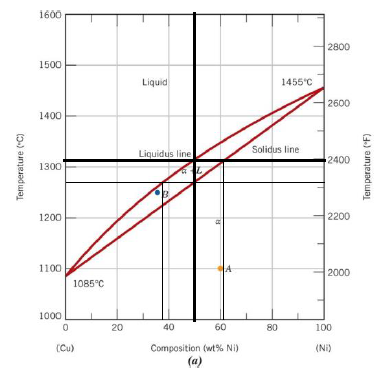
\includegraphics[width = 0.75\linewidth]{pro1.png}% Here is how to import EPS art
%	\caption{\label{fig:pro1} \ch{Ni-Co} Phase Diagram}
%	\end{centering}
%\end{figure}

\end{document}